\documentclass[twoside]{mfitjournal}
\usepackage{amsbib}
\clubpenalty=10000
\widowpenalty=10000
\newcommand{\MFITnumber}{}
\newcommand{\MFITom}{}
\newcommand{\MFITyear}{2026}
\newcommand{\ISSN}{}
\newcommand{\OISSN}{}
\newcommand{\DOI}{}
\renewcommand{\firstpage}{}
\renewcommand{\lastpage}{}
\SECC{}
\ESECC{}

\usepackage[T2A]{fontenc}
\usepackage[utf8]{inputenc}
\usepackage[russian]{babel}
\usepackage{amsmath,amssymb}
\usepackage{graphicx}
\usepackage{geometry}
\usepackage{booktabs}
\usepackage{caption}
\usepackage{float}
\usepackage{needspace}
\geometry{margin=2cm}
\setlength{\headheight}{15pt}
\captionsetup{font=small, labelfont=bf}

\begin{document}

\rustitle{Изучение дифракции света}
\shorttitle{Лабораторная работа 4.3.1}
\author{Иванов~Е.\,С.}
\shortauthor{Иванов~Е.\,С.}
\institute{МФТИ, группа Б05-407}
\email{}{}
\rcopyr{Иванов~Е.\,С.}

\makeatletter
\renewcommand{\tit}{}
\renewcommand{\@oddhead}{}
\renewcommand{\@evenhead}{}
\makeatother

\pagestyle{fancy}
\fancyhf{}
\fancyhead[RE]{Иванов~Е.\,С.}
\fancyhead[LO]{Лабораторная работа 4.3.1}
\cfoot{\arabic{page}}

\maketitle

% ======================================================
\section*{Цель работы}
% ======================================================

Изучить дифракцию Френеля и Фраунгофера на щели; определить длину волны
лазерного излучения по числу зон Шустера.

% ======================================================
\section*{В работе используются}
% ======================================================

Лазер, регулируемая щель ($d_1$ для Френеля, $d_2$ для Фраунгофера),
короткофокусная собирающая линза, микроскоп с объективом 4$\times$,
цифровая камера, оптическая скамья, калибровочная шкала.

% ======================================================
\section*{Теоретическая сводка}
% ======================================================

\textbf{Режимы дифракции.}
Характер дифракции на щели шириной~$b$ определяется волновым параметром
\begin{equation}\label{eq:wp}
    p = \frac{\sqrt{\lambda z}}{b},
\end{equation}
где $z$~--- расстояние от щели до плоскости наблюдения.
При $p \sim 1$ реализуется \emph{дифракция Френеля} (ближняя зона),
при $p \gg 1$~--- \emph{дифракция Фраунгофера} (дальняя зона).

\textbf{Дифракция Френеля на щели.}
Для анализа фреснелевской картины используется спираль Корню.
Вклад каждой узкой полоски щели изображается вектором на комплексной
плоскости; по мере удаления от центральной оси фаза нарастает
квадратично, и суммарный вектор закручивается в спираль.
Границы зон Шустера соответствуют полувиткам спирали; $m$-я граница
находится на расстоянии $\xi_m = \sqrt{m\lambda z}$ от оси.
Для симметричной щели, в центре которой укладывается ровно $m$~зон
Шустера на каждую полуширину, ширина щели равна
\begin{equation}\label{eq:fresnel}
    b = 2\sqrt{m\lambda z}.
\end{equation}
Отсюда при известном~$b$ можно определить~$\lambda$:
\begin{equation}\label{eq:lambda}
    \lambda = \frac{b^2}{4mz}.
\end{equation}
На графике $z(1/m)$ зависимость~(\ref{eq:fresnel}) линейна и проходит
через начало координат с наклоном $C = b^2/(4\lambda)$.
Число полос $m$ и расстояние $z$ связаны монотонно: чем ближе экран к
щели, тем больше зон Шустера укладывается в её ширине.

\textbf{Дифракция Фраунгофера на щели.}
В режиме $p\gg 1$ (практически реализуемом с помощью линзы) распределение
интенсивности в фокальной плоскости линзы с фокусным расстоянием~$f$
описывается формулой
\begin{equation}\label{eq:sinc}
    I(\theta) = I(0)\left(\frac{\sin\!\left(\dfrac{\pi b \sin\theta}{\lambda}\right)}
                                {\dfrac{\pi b \sin\theta}{\lambda}}\right)^{2}.
\end{equation}
Минимумы интенсивности ($I = 0$) отвечают условию $b\sin\theta_n = n\lambda$,
откуда их координаты в фокальной плоскости:
\begin{equation}\label{eq:fraun}
    x_n = f\tg\theta_n \approx n\frac{\lambda f}{b}, \quad n = 1,\,2,\,3,\ldots
\end{equation}
Расстояние между соседними минимумами $\Delta x = \lambda f / b$ постоянно
и не зависит от порядка $n$.

% ======================================================
\section*{Ход работы}
% ======================================================

\needspace{6\baselineskip}
\subsection*{1.\ Дифракция Френеля на щели}

Ширина щели измерена через камеру с объективом 4$\times$
(калибровка: $1\text{ мм} = 912.11\text{ пкс}$):
\[
    b = \frac{217\text{ пкс}}{912.11\text{ пкс/мм}} = 0{,}238\text{ мм.}
\]
При различных расстояниях~$z$ (отсчитанных от положения резкого
изображения щели $z_0 = 1{,}7$~мм) подсчитывалось число тёмных полос~$m$
во фреснелевской картине.
Качественные наблюдения подтверждают теорию: при уменьшении ширины щели
расстояние между дифракционными полосами не меняется, а при удалении
микроскопа число полос убывает.

Результаты измерений и значения~$\lambda$, вычисленные по формуле~(\ref{eq:lambda}),
приведены в Табл.~\ref{tab:fresnel}.

\begin{table}[htb]
\centering
\caption{Дифракция Френеля: число полос и расстояние до щели.
    Точка $m=1$ является выбросом и не включена в аппроксимацию.}\label{tab:fresnel}
\footnotesize
\begin{tabular}{cccc}
\toprule
$m$ & $z$, мм & $mz$, мм & $\lambda_i$, нм \\
\midrule
1 & 14{,}04 & 14{,}0 & 1008 \\
2 & 10{,}90 & 21{,}8 & 649 \\
3 &  7{,}69 & 23{,}1 & 613 \\
4 &  6{,}11 & 24{,}4 & 579 \\
5 &  5{,}13 & 25{,}7 & 552 \\
6 &  4{,}38 & 26{,}3 & 538 \\
\bottomrule
\end{tabular}
\end{table}

Аномальное значение $\lambda_1 \approx 1008$~нм при $m=1$ объясняется
трудностью однозначного определения ровно одной тёмной полосы при большом~$z$,
когда картина размыта.
Точка $m=1$ исключена из аппроксимации.

По точкам $m = 2{-}6$ проведён МНК-прямой через начало координат:
$z = C\cdot(1/m)$.
По наклону $C = 23{,}0 \pm 0{,}7$~мм определена длина волны:
\[
    \lambda = \frac{b^2}{4C}
    = \frac{(0{,}238)^2}{4 \times 23{,}0}
    = 616\text{ нм}.
\]

\begin{figure}[htb]
    \centering
    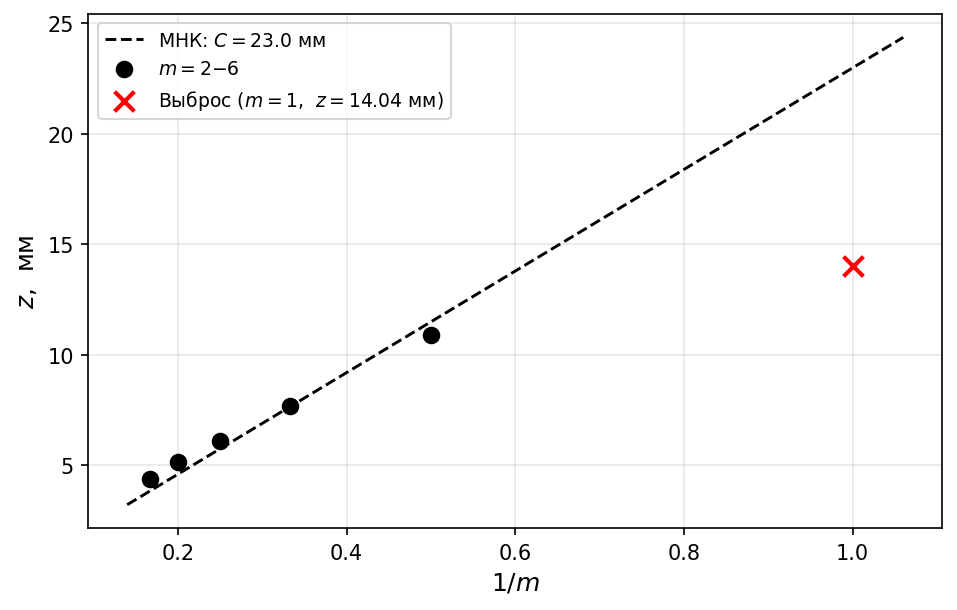
\includegraphics[width=0.82\linewidth]{fresnel_fit.png}
    \caption{Рис.~1. Зависимость $z$ от $1/m$. Пунктир~--- МНК-прямая
        по точкам $m=2{-}6$. Крест~--- выброс ($m=1$).}\label{fig:fresnel}
\end{figure}

На рис.~\ref{fig:fresnel} видно, что точки $m = 2{-}6$ хорошо ложатся на
прямую, а произведение $mz$ монотонно растёт от~21{,}8 до~26{,}3~мм.
Расхождение от идеального постоянства $mz = \mathrm{const}$ связано
с дискретностью отсчёта числа полос и погрешностью позиционирования
микроскопа.

С учётом погрешности ширины щели ($\delta b \approx 5$~пкс) и МНК:

\[
    \boxed{\lambda = (616 \pm 34)\text{ нм}.}
\]

\needspace{6\baselineskip}
\subsection*{2.\ Дифракция Фраунгофера на щели}

Параллельный пучок лазера пропускался через щель шириной~$b$, затем
фокусировался линзой на камеру.
В фокальной плоскости линзы зафиксированы координаты пяти минимумов
(Табл.~\ref{tab:fraun}).

\begin{table}[htb]
\centering
\caption{Дифракция Фраунгофера: координаты минимумов.}\label{tab:fraun}
\footnotesize
\begin{tabular}{ccc}
\toprule
$n$ & $x_n$, пкс & $x_n$, мм \\
\midrule
1 & 155{,}0 & 0{,}1700 \\
2 & 205{,}0 & 0{,}2249 \\
3 & 255{,}5 & 0{,}2802 \\
4 & 307{,}0 & 0{,}3367 \\
5 & 356{,}5 & 0{,}3909 \\
\bottomrule
\end{tabular}
\end{table}

Наблюдения подтверждают теорию: смещение щели поперёк оси не влияет на
картину, а увеличение ширины щели~$d_2$ сужает дифракционный максимум.

МНК по формуле~(\ref{eq:fraun}) даёт наклон
$\Delta x = (5{,}54 \pm 0{,}02)\times 10^{-2}$~мм ($R^2 = 0{,}9999$).

\begin{figure}[htb]
    \centering
    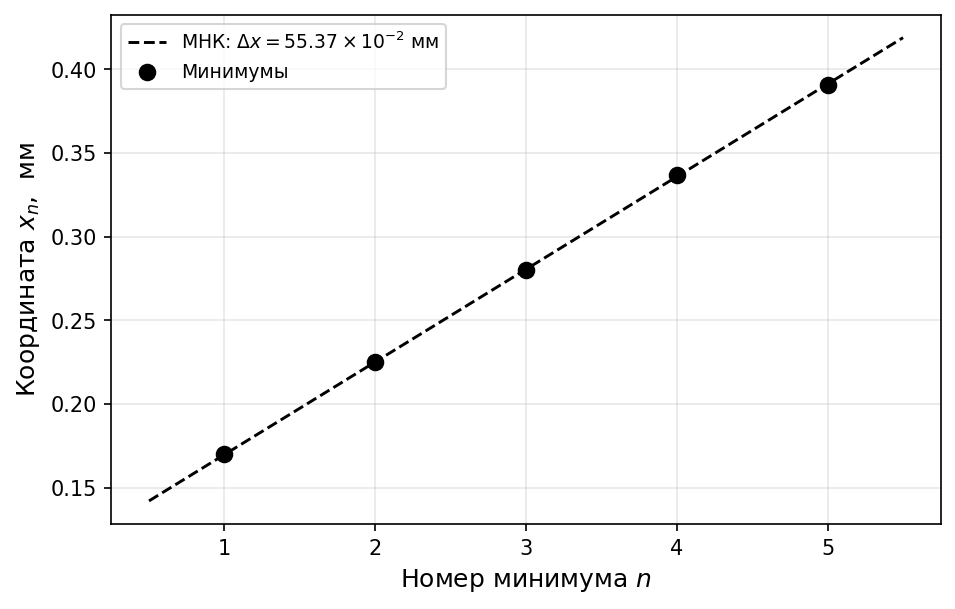
\includegraphics[width=0.82\linewidth]{fraunhofer_fit.png}
    \caption{Рис.~2. Координата $n$-го минимума $x_n$ в зависимости от
        номера~$n$. Пунктир~--- линейный МНК.}\label{fig:fraun}
\end{figure}

Поскольку $\Delta x = \lambda f / b$, используя $\lambda = 616$~нм
из п.~1 и $b = 0{,}238$~мм, получаем фокусное расстояние линзы:
\[
    f = \frac{\Delta x \cdot b}{\lambda}
    = \frac{5{,}54\!\times\!10^{-2} \times 0{,}238}{6{,}16\!\times\!10^{-4}}
    = 21{,}4\text{ мм.}
\]

% ======================================================
\section*{Вывод}
% ======================================================

\begin{enumerate}
    \item \textbf{Дифракция Френеля на щели.}
        По зависимости $z(m)$ при $m = 2{-}6$ (ширина щели
        $b = 0{,}238$~мм) методом МНК определена длина волны лазерного
        излучения: $\lambda = (616 \pm 34)$~нм.
        Значение соответствует видимому красно-оранжевому диапазону.
        Точка $m = 1$ является выбросом вследствие трудности однозначного
        отсчёта полос при большом~$z$.

    \item \textbf{Дифракция Фраунгофера на щели.}
        Координаты пяти минимумов линейно зависят от номера ($R^2 = 0{,}9999$),
        что подтверждает формулу~(\ref{eq:fraun}).
        Используя $\lambda$ из п.~1, найдено фокусное расстояние
        линзы $f = 21{,}4$~мм.
\end{enumerate}

\begin{thebibliography}{9}
\bibitem{desc}
    Копнин С.\,И., Пауков М.\,И., Пряжников А.\,Г.
    \textit{Лабораторная работа 4.3.1. Изучение дифракции света.}
    МФТИ, 2025.
\end{thebibliography}

\end{document}
